\documentclass[margin=1cm]{standalone}
\usepackage{tikz}
\usetikzlibrary{intersections}
\begin{document}
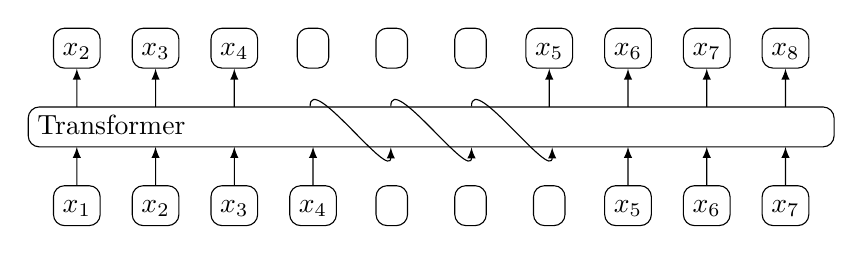
\begin{tikzpicture}[rounded corners, text height=1.5ex, text depth=0.3ex]
  \node[draw, text width=10cm, name path=tfmrborder] (tfmr) at (5.5,1) {Transformer};
  \foreach \timestep [
    count=\pos,
    remember=\timestep as \prevtstep (initially x_1)
  ] in {x_2,x_3,x_4,,,,x_5,x_6,x_7,x_8} {
    \node[
      draw,
      minimum size=4mm,
    ] (inpt\pos) at (\pos, 0) {\(\prevtstep\)};
    \node[
      draw,
      minimum size=4mm,
    ] (outpt\pos) at (\pos, 2) {\(\timestep\)};
  }
  \foreach \label in {1,2,3,7,8,9,10} {
    \path [name path=thru] (inpt\label) -- (outpt\label);
    \draw [name intersections={of=tfmrborder and thru, by={out, in}}, -latex] (out) -- (outpt\label);
  }
  \foreach \label in {1,2,3,4,8,9,10} {
    \path [name path=thru] (inpt\label) -- (outpt\label);
    \draw [name intersections={of=tfmrborder and thru, by={out, in}}, -latex] (inpt\label) -- (in);
  }
  \foreach \pos [
    count=\label,
    remember=\pos as \prevpos (initially 0.35)
  ] in {0.45,0.55,0.65} {
    \path (tfmr.north west) -- 
    coordinate[pos=(\label + 2.5) / 10] (out\label) 
    (tfmr.north east);
    \path (tfmr.south west) -- 
    coordinate[pos=\pos] (in\label) 
    (tfmr.south east);
    \draw[-latex] (out\label) to[out=north, in=south] (in\label);
  }
\end{tikzpicture}
\end{document}
